\begin{center}
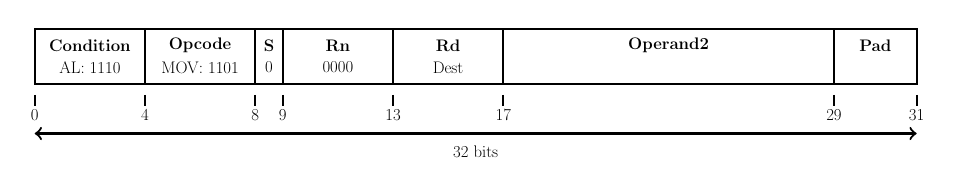
\begin{tikzpicture}[scale=0.35, every node/.style={scale=0.35}]
    % Bit fields with adjusted widths and labels for clarity
    \draw[thick] (0,0) rectangle (4,2) node[midway, yshift=0.4cm] {\textbf{\LARGE Condition}};
    \node at (2, 0.6) {\LARGE AL: 1110};
    
    \draw[thick] (4,0) rectangle (8,2) node[midway, yshift=0.4cm] {\textbf{\LARGE Opcode}};
    \node at (6, 0.6) {\LARGE MOV: 1101};
    
    \draw[thick] (8,0) rectangle (9,2) node[midway, yshift=0.4cm] {\textbf{\LARGE S}};
    \node at (8.5, 0.6) {\LARGE 0};
    
    \draw[thick] (9,0) rectangle (13,2) node[midway, yshift=0.4cm] {\textbf{\LARGE Rn}};
    \node at (11, 0.6) {\LARGE 0000};
    
    \draw[thick] (13,0) rectangle (17,2) node[midway, yshift=0.4cm] {\textbf{\LARGE Rd}};
    \node at (15, 0.6) {\LARGE Dest};
    
    \draw[thick] (17,0) rectangle (29,2) node[midway, yshift=0.4cm] {\textbf{\LARGE Operand2}};
    
    \draw[thick] (29,0) rectangle (32,2) node[midway, yshift=0.4cm] {\textbf{\LARGE Pad}};
    
    % Bit numbers
    \draw[thick] (0,-0.4) -- (0,-0.8) node[below] {\LARGE 0};
    \draw[thick] (4,-0.4) -- (4,-0.8) node[below] {\LARGE 4};
    \draw[thick] (8,-0.4) -- (8,-0.8) node[below] {\LARGE 8};
    \draw[thick] (9,-0.4) -- (9,-0.8) node[below] {\LARGE 9};
    \draw[thick] (13,-0.4) -- (13,-0.8) node[below] {\LARGE 13};
    \draw[thick] (17,-0.4) -- (17,-0.8) node[below] {\LARGE 17};
    \draw[thick] (29,-0.4) -- (29,-0.8) node[below] {\LARGE 29};
    \draw[thick] (32,-0.4) -- (32,-0.8) node[below] {\LARGE 31};

    % Arrow for full bit length label
    \draw[<->, thick] (0,-1.8) -- (32,-1.8) node[midway, below, yshift=-0.3cm] {\LARGE 32 bits};
\end{tikzpicture}
\end{center}
